Muon efficiencies are measured with the Tag-and-Probe method performed on
$\cPZ \to \Pgm\Pgm$ and $\JPsi\to\mu\mu$ events in bins of $\pt$ and $\eta$. 
% More
%details on the methodology can be found in Ref.~\cite{CMS_AN_2015-277}. Measurements are extracted using 2018 RunA,B,C,D data while the measurements corresponding to 2016 and 2017 datasets have already been reported in Ref.~\cite{CMS_AN_2016-442} and Ref.~\cite{CMS_AN_2017-342} respectively.
%
The $\Z$ sample is used to measure the muon reconstruction and identification efficiency at high $\pt$,
and the efficiency of the isolation and impact parameter requirements at all $\pt$.
%
The $\JPsi$ sample is used to measure the reconstruction efficiency at low $\pt$,
as it benefits from a better yield in that kinematic regime.
In this case, events are collected using triggers that require a muon with $\pt > 7.5\GeV$
and an additional track (muon) with $\pt > 2 \GeV$ when probing the reconstruction (tracking) efficiency.

Results for the muon reconstruction and identification efficiency for $\pt > 20\GeV$
have been derived by the CMS collaboration.
The probe in this measurement are tracks reconstructed in the inner tracker, and
the passing probes are those that are also reconstructed as a global or tracker muon 
and pass the identification criteria.
%
Results for low \pt muons were derived using \JPsi events, with the same definitions
of probe and passing probes. The systematic uncertainties are estimated by varying the analytical signal and background shape models used to fit 
the dimuon invariant mass. 
% Details on the procedure can be found in Ref.~\cite{AN-15-277}. 
The efficiency and scale 
factors used for low $\pt$ muons are the ones derived using single muon dataset.

For the impact parameter requirements, the measurement is performed using $\Z$ events.
Events are selected with single muon triggers requiring an isolated muon with $\pt > 27\GeV$ or a muon with $\pt > 50 \GeV$.
For this measurement, the probe is a muon passing the identification criteria,
and it is considered a passing probe if satisfies the \SIPthreeD, $d_{xy}$ and $d_z$ cuts of this analysis.
%
The efficiency to reconstruct a muon track in the inner detector is measured using as probes tracks
reconstructed in the muon system alone. The efficiency and 
data to MC scale factors are measured from Z events as a function of $\eta$ and \pt.
The scale factors are shown in Figure~\ref{fig:muoSFRun2}.

\begin{figure}
  \centering
  \subfigure [2016] {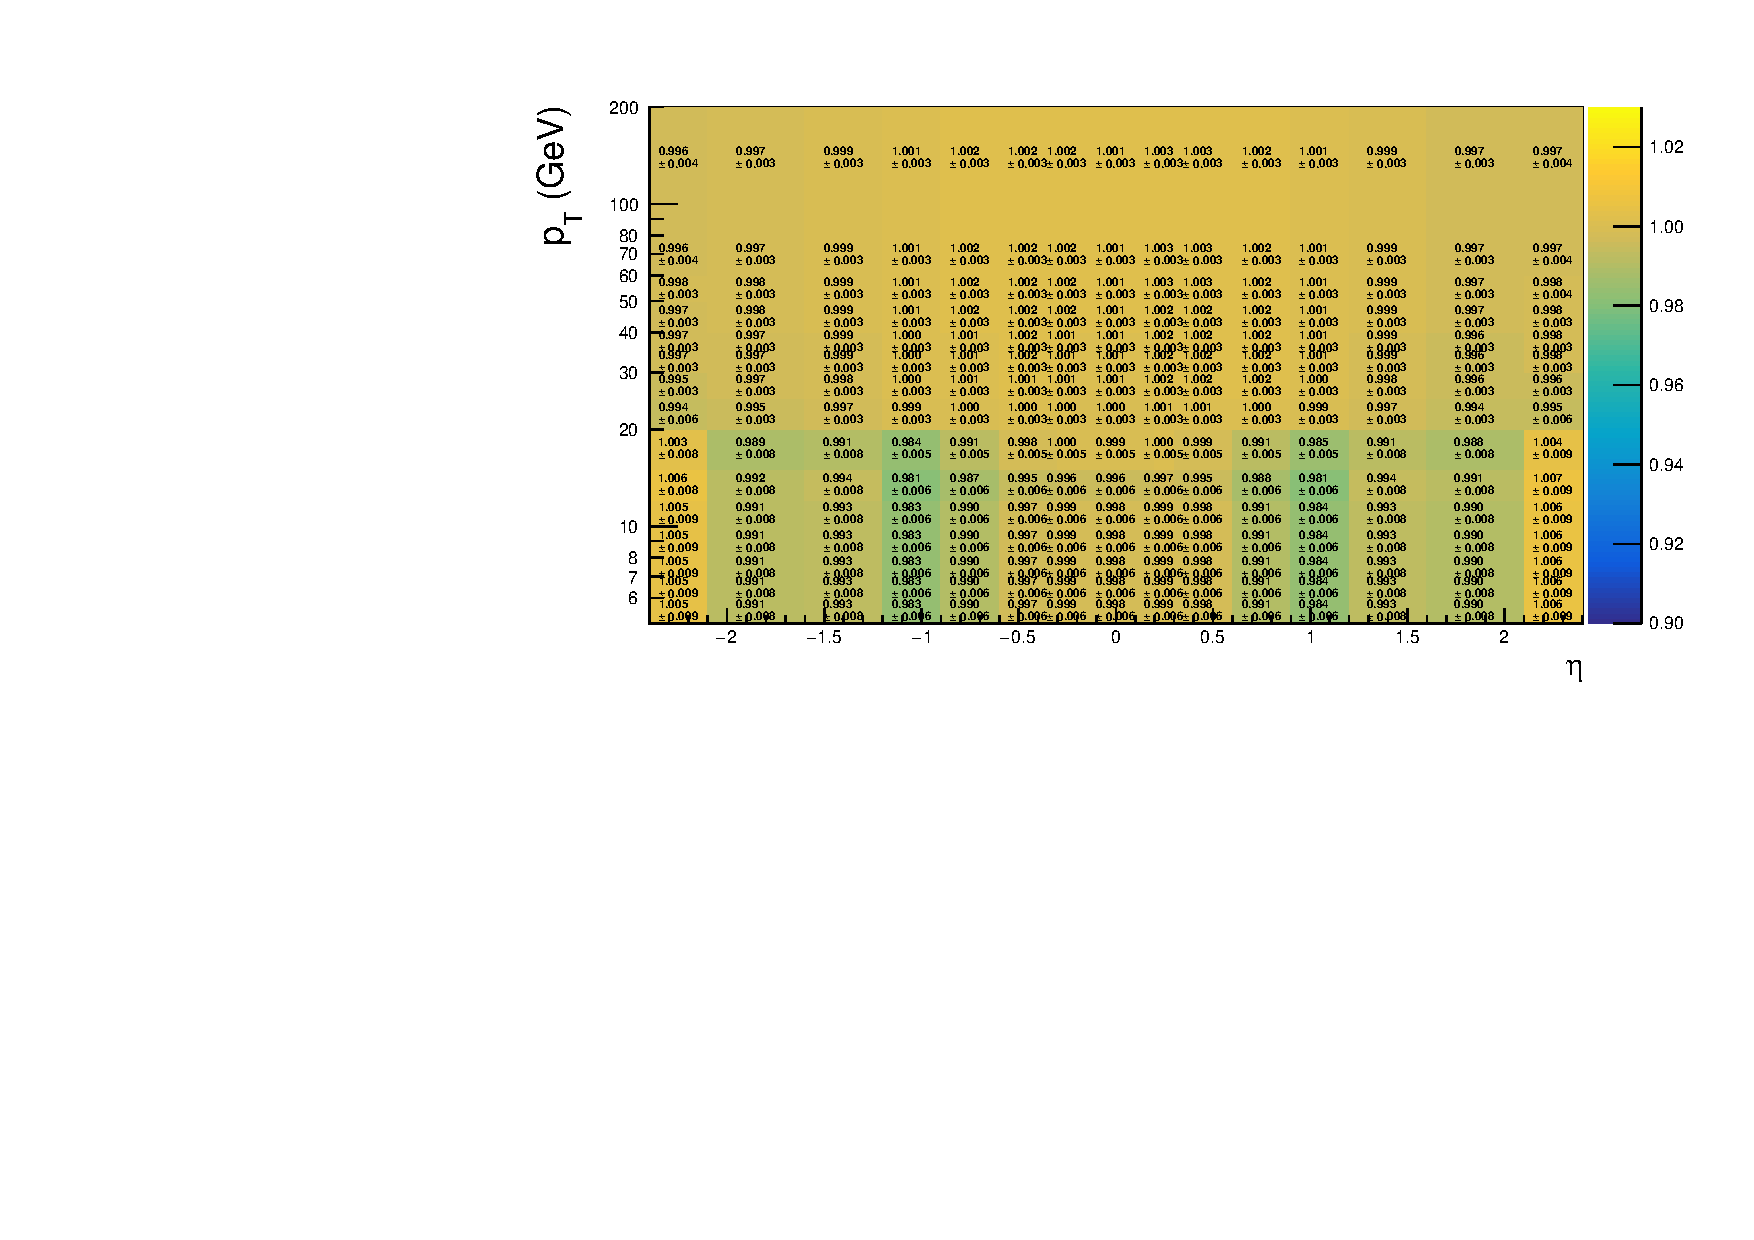
\includegraphics[height=.25\textheight]{final_HZZ_SF_2016UL_mupogsysts_newLoose_FINAL.pdf}}\\
  \subfigure [2017] {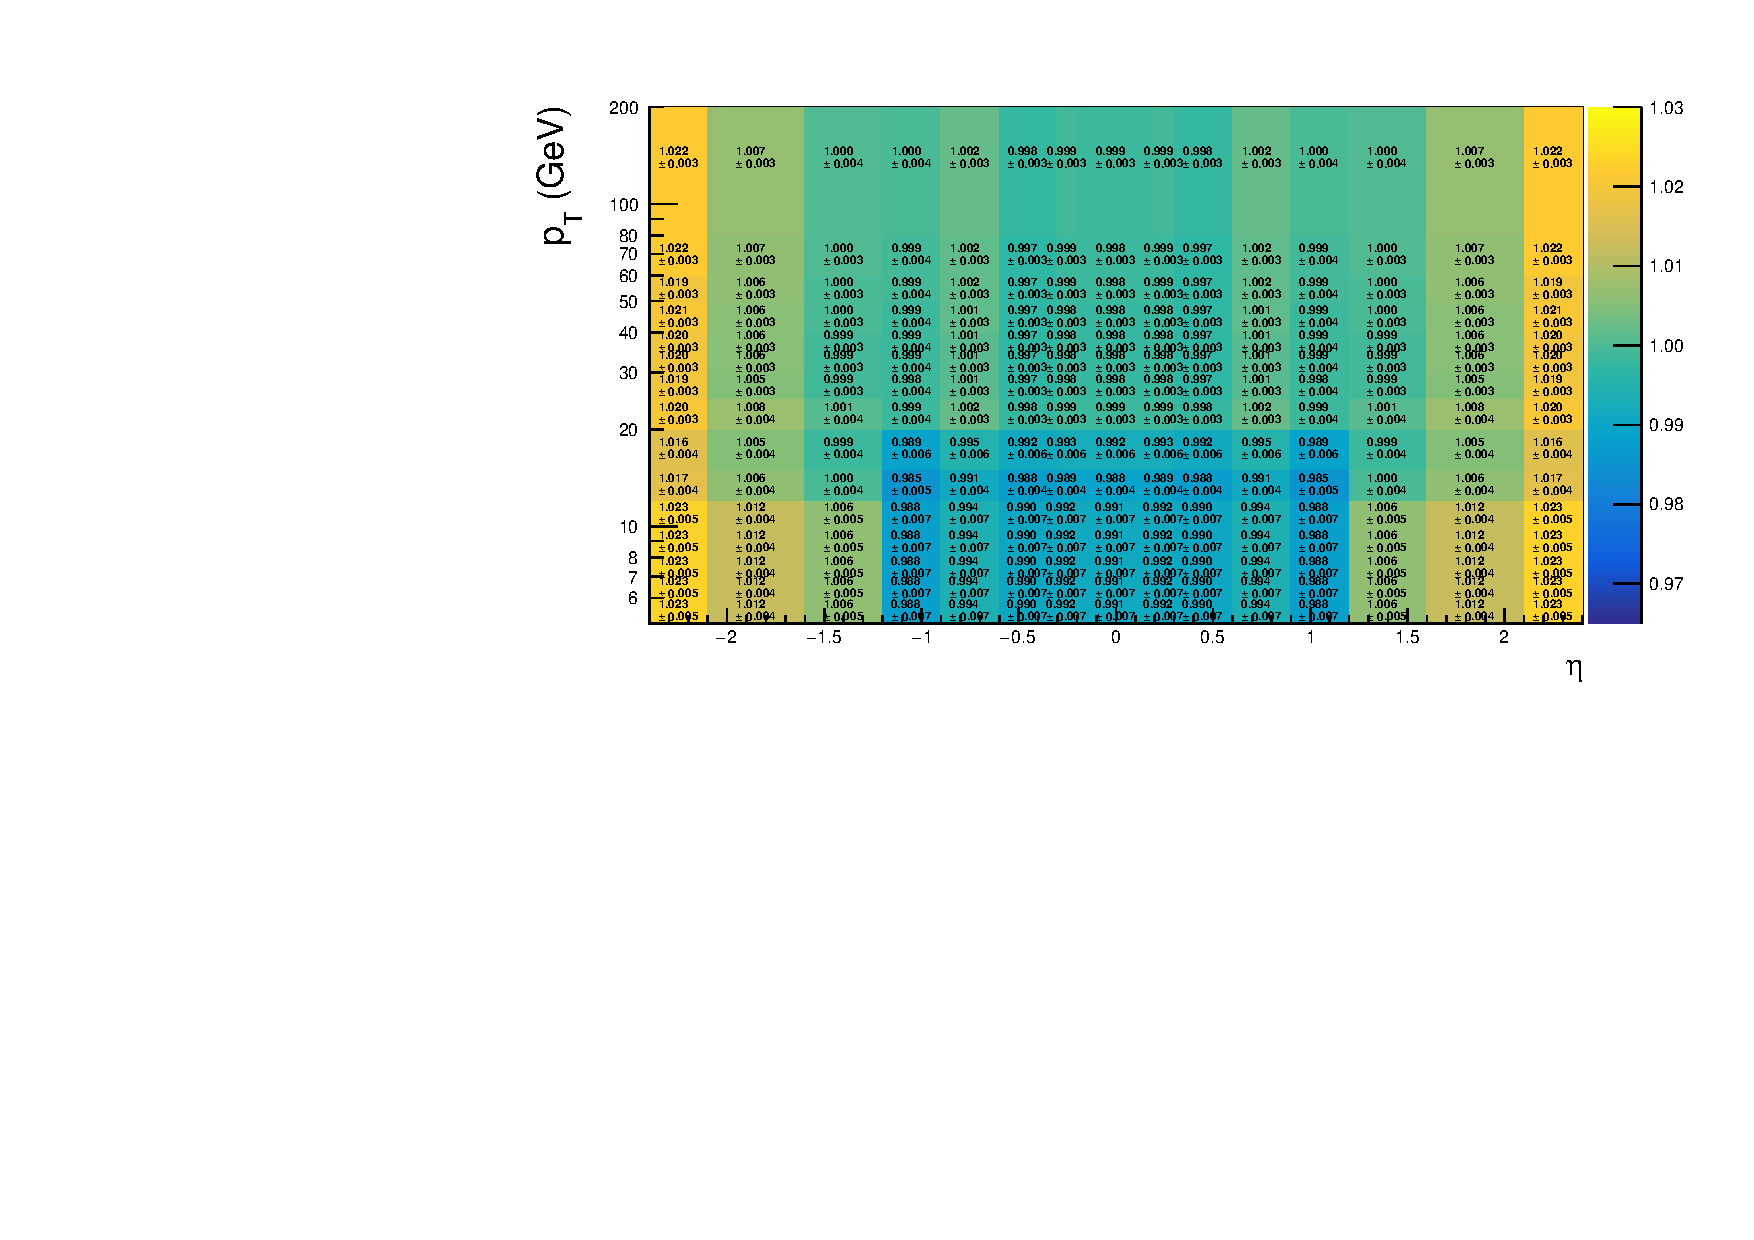
\includegraphics[height=.25\textheight]{final_HZZ_SF_2017UL_mupogsysts_newLoose_FINAL.pdf}}\\
  \subfigure [2018] {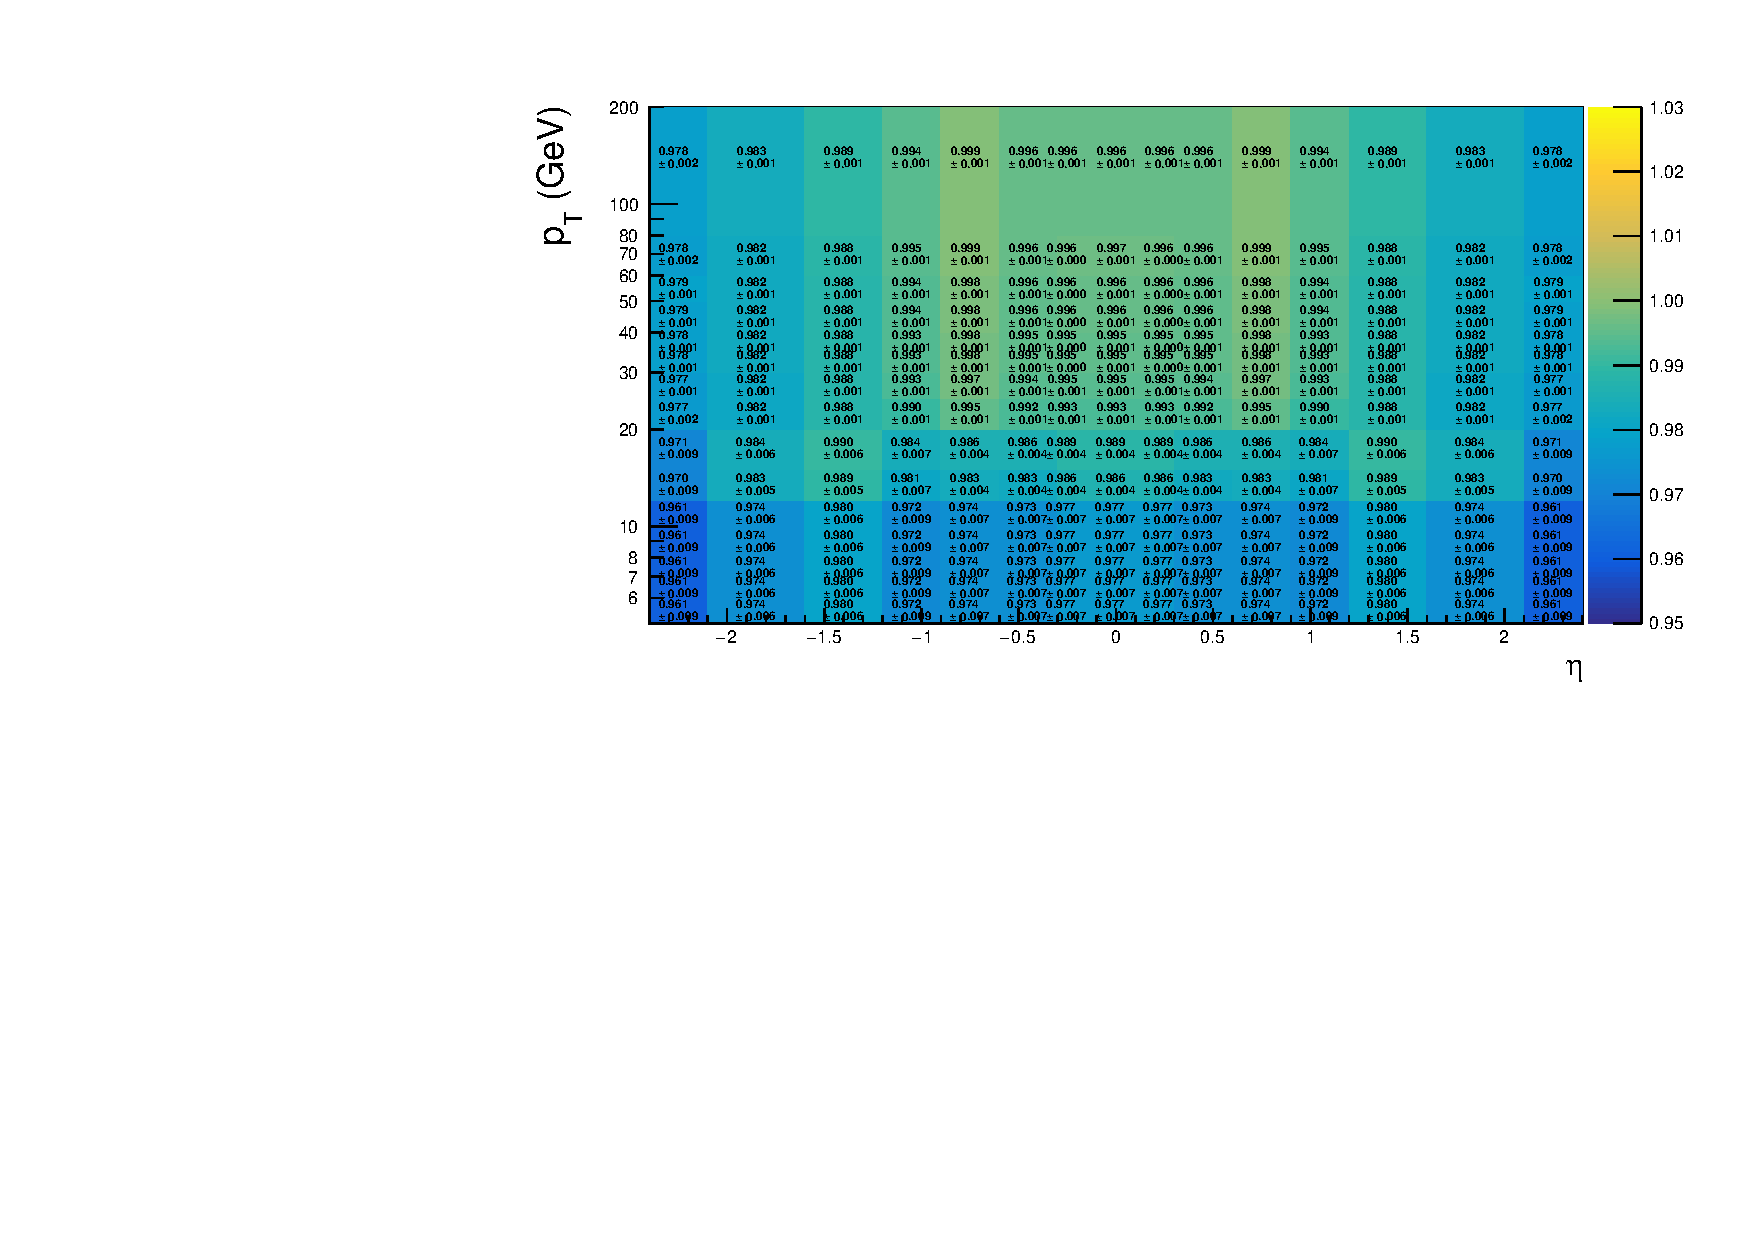
\includegraphics[height=.25\textheight]{final_HZZ_SF_2018UL_mupogsysts_newLoose_FINAL.pdf}}
  \caption{Efficiency scale factors, calculated as ratio between the efficiency in data and in simulation,
  applied to muons for the three years of data taking in \RunII.}
  \label{fig:muoSFRun2}
\end{figure}
